\chapter{FUNDAMENTAÇÃO TEÓRICA}

Neste capítulo serão abordados conceitos relacionados a Sistemas Distribuídos e os recursos necessários para realizar balanceamento de carga, tendo forte embasamento nos autores \citeauthoronline{Tanenbaum} e \citeauthoronline{Coulouris-2012} que são de grande renome no âmbito de sistemas distribuídos.

\section{Sistemas Distribuídos}
	%Introduzir as definições explicando que vou utilizar de dois autores, blablabal

	Graças aos grandes avanços tecnológicos no decorrer dos últimos 50 anos, tornou-se possível criar sistemas compostos por inúmeros computadores ligados por uma rede de alta velocidade, também conhecidos como sistemas distribuídos. Estes podem ser definidos como um conjunto de computadores independentes que se apresenta a seus usuários como um sistema único e coerente \cite{Tanenbaum}.
	
	Segundo \citeauthoronline{Coulouris-2012} (\citeyear{Coulouris-2012}) um sistema distribuído consiste em um conjunto de componentes de \textit{softwares} e/ou \textit{hardwares} conectados em uma rede de computadores que são capazes de organizar suas ações somente pela troca de mensagens.
	
	Sistemas distribuídos são então, um conjunto de componentes computacionais independentes conectados por uma rede em que, a partir da troca de mensagens, representam um único sistema para o usuário final.
	
	Os computadores e programas que compõe um sistema são autônomos e se apresentam aos usuários ou programas como um sistema único, o que implica em uma colaboração entre eles, a forma como se estabelece esta colaboração é a questão mais importante do sistema \cite{Tanenbaum}. 
	
	Uma característica forte nos sistemas distribuídos é ser heterogêneo, ou seja, ser composto por diferentes \textit{hardwares}, sistemas operacionais e \textit{softwares} de variadas linguagens de programação. Estas diferenças e a forma de comunicação entre elas é oculta ao usuário. Expandir a quantidade de máquinas também deverá ser possível, sendo que cada máquina é autônoma, isto serve principalmente para que a aplicação possa continuar executando mesmo com algum computador avariado \cite{Tanenbaum}.
	
	A transparência do sistema, ou seja, ocultar que os recursos e processos estão ocorrendo em máquinas diferentes é uma das principais metas dos sistemas distribuídos. Este conceito está ligado a diversos aspectos do sistema, podendo ser resumido nas transparências apresentadas na tabela \ref{transparencia}.
	
	\begin{table}[]
		\caption{Formas de transparência em sistemas distribuídos.}
		\label{transparencia}
		\fonte{
			\citeauthoronline{Tanenbaum} 
			\citeyear{Tanenbaum}
		}
		\begin{tabularx}{\linewidth}{|l|m|}
			\hline
			\textbf{Transparência} & \textbf{Descrição} \\ \hline
			Acesso & Oculta diferenças na representação de dados e no modo de acesso a um recurso \\ \hline
			Localização & Oculta o lugar em que um recurso está localizado \\ \hline
			Migração & Oculta que um recurso pode ser movido para outra localização \\ \hline
			Relocação & Oculta que um recurso pode ser movido para uma outra localização enquanto em uso \\ \hline
			Replicação & Oculta que um recurso é replicado \\ \hline
			Concorrência & Oculta que um recurso pode ser compartilhado por diversos usuários concorrentes \\ \hline
			Falha & Oculta a falha e a recuperação de um recurso \\ \hline
		\end{tabularx}
	\end{table}
	
	No trabalho serão abordados principalmente dois conceitos, transparência de acesso que oculta as diferenças de arquitetura das máquinas, fazendo com que sistemas operacionais diferentes possam se comunicar de forma padrão e tornem suas diferenças imperceptíveis. E transparência de localização que faz com que o usuário desconheça o local físico em que um recurso se encontra. 
	
	Uma das formas de obter transparência e então fazer a conexão entre as máquinas de diferentes sistemas operacionais, aplicações e localizações em um sistema único, é a partir da utilização de \textit{middlewares}. 
	
	\subsection{Middleware}
	O termo \textit{middleware} esta relacionado a uma camada de \textit{software} que torna possível a programação abstrata e mascarar as diferenças de \textit{hardware}, sistema operacional e linguagens de programação dos componentes que fazem parte do sistema distribuído. Cada \textit{middleware} tem suas próprias características, alguns suportam apenas uma linguagem de programação, invocação de objetos ou eventos remotamente, entre outras \cite{Coulouris-2012}.
	
	É representado por processos ou objetos em um conjunto de computadores que se comunicam e compartilham recursos para aplicações distribuídas \cite{Coulouris-2012}. A Figura \ref{fig:Tanenbaum-middleware} apresenta quatro máquinas autônomas que são responsáveis por aplicações somente suas ou compartilhadas, a comunicação entre estas máquinas heterogêneas é coordenada pelo \textit{middleware}. 
		
	\begin{figure}[htb]
		\caption{Atuação da camada \textit{middleware}}
		{\parbox{6cm}{
				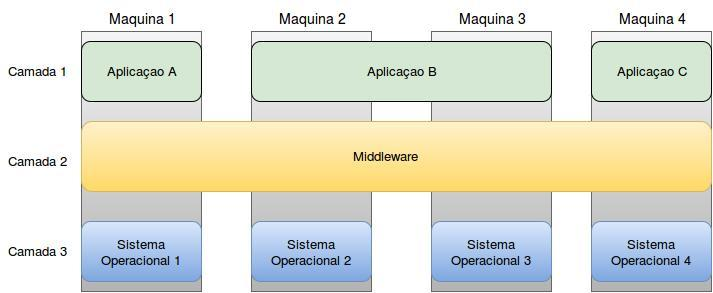
\includegraphics[width=14cm]{images/middleware.jpeg}
				\label{fig:Tanenbaum-middleware}
				\fonte{
					\citeauthoronline{Tanenbaum} 
					\citeyear{Tanenbaum}
				}
		}}
	\end{figure}

	Sistemas de \textit{middleware} costumam seguir um estilo arquitetônico específico, CORBA segue um estilo baseado em objetos, enquanto TIB/Rendezvous foi desenvolvido para arquitetura baseadas em evento. Usar uma arquitetura específica como molde simplifica o projeto de aplicações.
	
	A orientação a objetos é um conceito forte no desenvolvimento de \textit{software} e foi utilizado para a criação de sistemas baseados em objetos distribuídos. Um objeto tem como característica o encapsulamento de dados e operações que podem ser utilizadas nestes, nos sistemas um cliente costuma ter somente uma interface que é a declaração das operações que podem ser executadas, enquanto o servidor guarda os objetos com a implementação das interfaces, os objetos. O servidor também contém um esqueleto, que fornece o mínimo necessário de meios para que o \textit{middleware} acesse os objetos.
	
	Os objetos em sistemas distribuídos existem em vários formatos, sendo a mais comum serem similares a objetos de linguagens de programação como C ou Java. Um dos principais \textit{middlewares} que aderiu esta ideia é o CORBA, o qual será alvo do desenvolvimento do trabalho.
	
	%Apresentar alguns middlewares (RMI, Rest, CORBA) e fazer um gancho para CORBA
\section{CORBA}
	O CORBA (\textit{Common Object Request Broker Architecture}) é uma arquitetura com a finalidade de permitir que objetos de sistemas distribuídos possam se comunicar de forma transparente entre si, sem depender de suas plataformas de hardware, sistemas operacionais e linguagem de programação na qual foram desenvolvidos. Hoje em dia, sem dúvida alguma, esta arquitetura é a melhor opção para desenvolver aplicações de interação de cliente/servidor (RICCIONI, 2003).
	
	O modelo tem como base três conceitos principais: integração e reuso de componentes, orientação a objetos e um ambiente de computação distribuído e aberto. A arquitetura CORBA utiliza o modelo cliente/servidor e também um mediador entre estes agentes visando reduzir a complexidade de sua interação. O mediador é conhecido como ORB (\textit{Object Request Broker}) e é responsável por localizar os objetos para qual se destinam as requisições da rede, além do envio dos parâmetros da requisição e de suas respectivas respostas, caso existam.

	CORBA é uma arquitetura que permite a interação entre objetos distribuídos em diferentes linguagens e sistemas, além de proporcionar maior transparência na comunicação entre os objetos. Para localizar os objetos são feitas referências que poderão ser resolvidas pelo ORB.
	
	Para descrever as interfaces dos objetos é utilizada a linguagem IDL (\textit{Interface Definition Language}), esta é uma linguagem que contém apenas declarações. Os tipos de dados são exclusivos da linguagem e são mapeados para tipos respectivos de acordo com as linguagens que ela suporta.
	
	Em um arquivo .idl é possível definir um módulo, neste serão inseridos todas as outras definições: tipos de dados, estruturas de dados, métodos, parâmetros e exceções. A partir deste arquivo é possível criar diversas interfaces com diferentes compiladores para diferentes linguagens.
	
	Uma vez que os arquivos java são gerados, é necessário que você implemente os métodos e exceções para que eles funcionem da forma desejada. Após implementar basta ambos servidor e  cliente utilizarem os objetos ORB para fazer a comunicação.

\section{Balanceamento de Carga}
	Diferente dos sistemas de máquina única, os sistemas distribuídos apresentam a possibilidade de falha parcial, ou seja, um dos componentes apresentar problemas enquanto os outros continuam estão trabalhando. Esta falha poderá afetar o processo de alguns componentes e de outros não, mas o projeto do sistema já deve prever esta possibilidade e ser construído de forma a manter-se funcionando até se recuperar automaticamente da falha.
	
	Tolerar falhas é um dos pontos mais importantes em sistemas distribuídos e segundo \citeauthoronline{Tanenbaum} (\citeyear{Tanenbaum}) "Há forte relação entre ser tolerante a falha e os denominados sistemas confiáveis". Para tal são alçados alguns requisitos: Disponibilidade, capacidade de um sistema estar pronto para uso a qualquer momento de forma imediata. Confiabilidade, capacidade de um sistema executar o máximo possível de tempo sem apresentar falhas. Segurança, ser capaz de assegurar que mesmo apresentando falhas nada de grave acontecerá. Capacidade de manutenção, facilidade com que as falhas no sistema são corrigidas automaticamente ou não.
	
	Sistemas apresentam defeitos quando não são capazes de fornecer aos usuários todos os serviços que deveriam. Erros podem ocorrer por diversos motivos, sendo suas causas conhecidas como falhas, tolerar elas significa que um sistema possa continuar funcionando mesmo na presença das mesmas. As falhas são classificadas como transientes quando acontecem uma vez e não se repetem mais, intermitentes se acontecem vez ou outra mas sem conhecimento do motivo ou permanentes quando continuam acontecendo até serem corrigidas.
	
	As falhas dentro de um sistema distribuído podem ser várias, podem ser no próprio componente ou no meio de transmissão visto que eles precisam se comunicar entre si. Para abstrair o conhecimento desta imensidão de possibilidades, pode-se classificar as falhas como queda, omissão de recebimento, omissão de envio, temporização, valor de resposta, transição de estado da resposta e arbitrárias.
	
	Uma das formas de tolerar falhas é as ocultando, sendo a redundância a principal técnica de ocultação de falhas. É possível realizar redundância por tempo que fará com que caso uma ação falhe seja executada novamente por um determinado tempo, redundância física onde novos componentes são adicionados para possibilitar que o sistema ignora o mal funcionamento de outro componente, e redundância de informação na qual alguns dados repetidos são adicionados a resposta para que esta possa ser recuperada em caso de falha na transmissão.
	
	Com isto foram criados os processos em grupos que tem seu funcionamento dado pela replicação de processos em grupos, ou seja, uma mesma funcionalidade do sistema é executada por todos os componentes de um conjunto e com as \textit{n} respostas geradas é possível tolerar e detectar falhas, pois se um falhar outro irá se encarregar de responder.
	
	Grupos de processos podem apresentar estruturas internas diferentes, grupos simples são os que todos os processos podem ser iguais e sem nenhum tomador de decisão, já os grupos hierárquicos tem um processo coordenador que organiza as tarefas e define qual processo irá executar cada tarefa. Ambos apresentam prós e contras, grupos simples continuam a funcionar normalmente com a queda de um dos membros mas as tomadas de decisões são mais complexas, já grupos hierárquicos tem facilidade na tomada de decisões mas são dependentes de um coordenador, se este falhar o grupo inteiro fica parado.
	
	Outro princípio fundamental é a segurança, que está fortemente relacionada com a confiabilidade. A segurança se apresenta como um dos tópicos mais complexos pela necessidade de estar presente em todo o sistema, uma única falha pode destruir toda a estrutura construída.
	
	É possível dividir a segurança em duas partes, a comunicação entre usuários ou processos e a autorização que assegura que um processo receba acesso somente aos recursos habilitados. Existem também quatro principais tipos de ameaças a segurança: interceptação ocorre quando um componente não autorizado consegue acesso a um serviço ou dados restritos, interrupção quando arquivos são corrompidos ou perdidos, modificação quando ocorre uma alteração não autorizada em dados e invenção quando são gerados dados  ou atividades adicionais que não deveriam existir.
	
	A utilização de canais seguros é essencial, estes irão fornecer os meios necessários para autenticar ambas as partes que estão se comunicando e também proteger as mensagens envidas contra modificação e leitura de membros exteriores. Outro ponto é a utilização de apenas um criptossistema simétrico ou até combinar este com um sistema de chave pública, também conhecidos como chave de sessão.
	
	O controle de acesso deve ser utilizado para que somente os processos com permissão tenham acesso aos recursos solicitados. Uma forma de implementar este controle é fazer que cada recurso mantenha uma lista com os processo que podem acessar, ou então emitir certificados para os processo indicando as permissões do mesmo.
	
\section{Containers}
	A ideia de dividir processos e intercalar sua execução de forma a parecerem simultâneos, que é muito comum em programação \textit{multithread}, é aplicada a virtualização de recursos que tende a simular múltiplos ambientes de \textit{hardware} e \textit{software} em um única máquina.
	
	É comum que os sistemas distribuídos ofereçam uma das várias interfaces de programação de software de alto nível, a virtualização substitui uma interface já existente para simular o comportamento de outro sistema. A real necessidade de virtualizar sistemas surgiu quando o \textit{hardware} começou a evoluir rapidamente na década de 90, mas os \textit{softwares} e \textit{middlewares} não acompanhavam o mesmo ritmo, simular os ambientes antigos colaborou para que a compatibilidade de sistemas fossem mantidas nas novas máquinas enquanto os programas evoluíam.
	
	A virtualização também surgiu para facilitar a manutenção dos administrados de sistemas, isto porque todo o sistema e suas configurações ficavam salvas e poderiam ser transportadas ou copiadas para uma nova máquina a qualquer momento.
	
	A partir das grandes vantagens em se utilizar virtualização para sistemas distribuídos, junto as rápidas evoluções de \textit{hardware} e redes de computador, tornou-se possível evoluir também na forma de virtualizar. Simular todo um sistema operacional pode custar muito caro pois muito tempo e processamento são desperdiçados com processos desnecessários, surgiu então a era dos \textit{containers}.
	
	\textit{Containers} são ambientes de execução criados para um programa específico, isolando o mesmo de todos os recursos do computador que não serão necessários para seu funcionamento. Os principais benefícios são a segurança por remover o acesso a recursos desnecessários, rápida execução por não precisar iniciar grande parte dos componentes de um sistema operacional e tornar o programa executável em qualquer computador por garantir que este sempre estará executando em um mesmo ambiente computacional.

	Diferente das máquinas virtuais os \textit{containers} não utiliza, da virtualização de \textit{hardware}, os programas se comunicam diretamente com o \textit{kernel} do Linux da máquina. Isso porque não são adicionadas camadas adicionais entre o \textit{container} e o sistema operacional para ganhar desempenho ao não desperdiçar recursos simulando um ambiente de hardware, essa diferença está apresentada na figura \ref{fig:Docker-container-vm}.

	\begin{figure}[htb]
		\caption{Diferença de camadas entre \textit{containers} e máquinas virtuais}
		{\parbox{6cm}{
				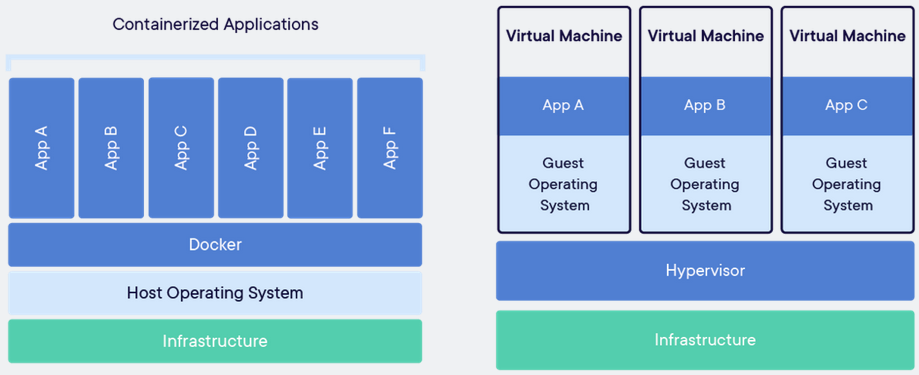
\includegraphics[width=15cm]{images/container_x_vm.png}
				\label{fig:Docker-container-vm}
				\fonte{
					https://www.docker.com/resources/what-container
					\citeyear{}
				}
		}}
	\end{figure}

	Apesar de vantagens apresentadas, a construção manual de um \textit{container} pode se apresentar devidamente complexa e portanto facilmente pode ser feita da forma incorreta, com erros de configuração e falhas de segurança. Para facilitar e padronizar a construção destes surgiu o Docker, que a partir de configurações próprias cria um \textit{container} dentro dos padrões e utilizando as melhores práticas de construção.
	%Ligar com o tema de SD, mobilidade de aplicação, transparência e etc.
\subsection{Docker}
	De uma forma simples é possível definir Docker como uma maneira de abranger diferentes serviços em ambientes isolados, que contém todos os recursos necessários para garantir ao desenvolvedor que o serviço irá funcionar em qualquer local que o Docker seja executado \cite{Hane}.
	
	Docker desenvolveu sua própria ferramenta de construção de \textit{containers}. Ao ser instalado na máquina(Linux ou Windows), disponibiliza uma interface de linha de comando que se comunica com um \textit{daemon} próprio, este é o responsável por organizar todas as instâncias em execução. Sendo assim, é considerado como um sistema para interagir com \textit{containers} no formato cliente-servidor, onde o terminal de comandos é o cliente e o \textit{daemon} o servidor. Na figura \ref{fig:Docker-daemon} está apresentado uma estrutura executando Docker, que por sua vez está com três instâncias simultâneas com suas próprias dependências, executando de forma isolada.
	
	\begin{figure}[htb]
		\caption{Execução de \textit{containers} utilizando Docker em um sistema operacional Linux comum}
		{\parbox{6cm}{
				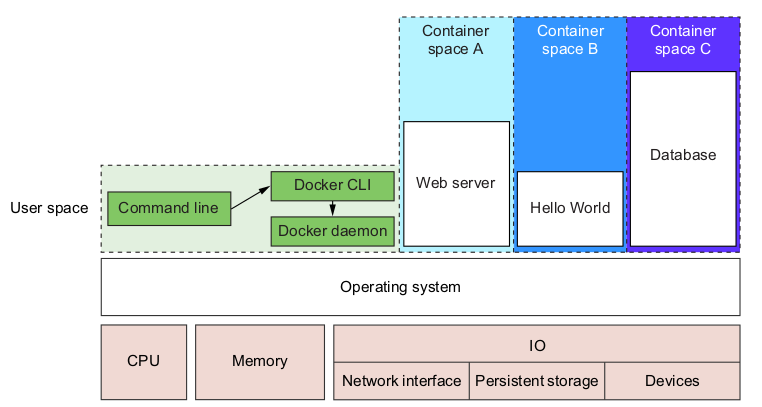
\includegraphics[width=15cm]{images/docker-daemon.png}
				\label{fig:Docker-daemon}
				\fonte{https://www.docker.com/resources/what-container}
		}}
	\end{figure}

O diferencial que o fez ganhar grande espaço no universo da tecnologia são as Imagens Docker, responsáveis por inicializar um \textit{container}. A imagem é um conjunto de instruções que define como deve ocorrer a criação do \textit{container} Docker, especificando qual ambiente computacional, bibliotecas e pacotes que devem ser instalados, comandos a serem executados, configurações de memória, processamento, rede, assim como a criação de espaços de armazenamento próprio ou compartilhado. Com elas o processo de reprodução e distribuição de um \textit{container} que antes era complicado se torna simples, ainda mais com o repositório de imagens (DockerHub) mantido pela empresa, onde qualquer usuário pode fazer \textit{upload} e \textit{download} de imagens.



